En diferentes entornos, existe una problemática en la que la gestión del inventario de productos se ve afectado debido a la falta de información precisa sobre la demanda mensual de los mismos, lo que dificulta la planificación adecuada del abastecimiento. En este contexto, surge la necesidad de contar con herramientas que permitan analizar los datos históricos de inventario y generar estimaciones de demanda que apoyen la toma de decisiones relacionadas con el abastecimiento.

\begin{figure}[H]
    \centering
    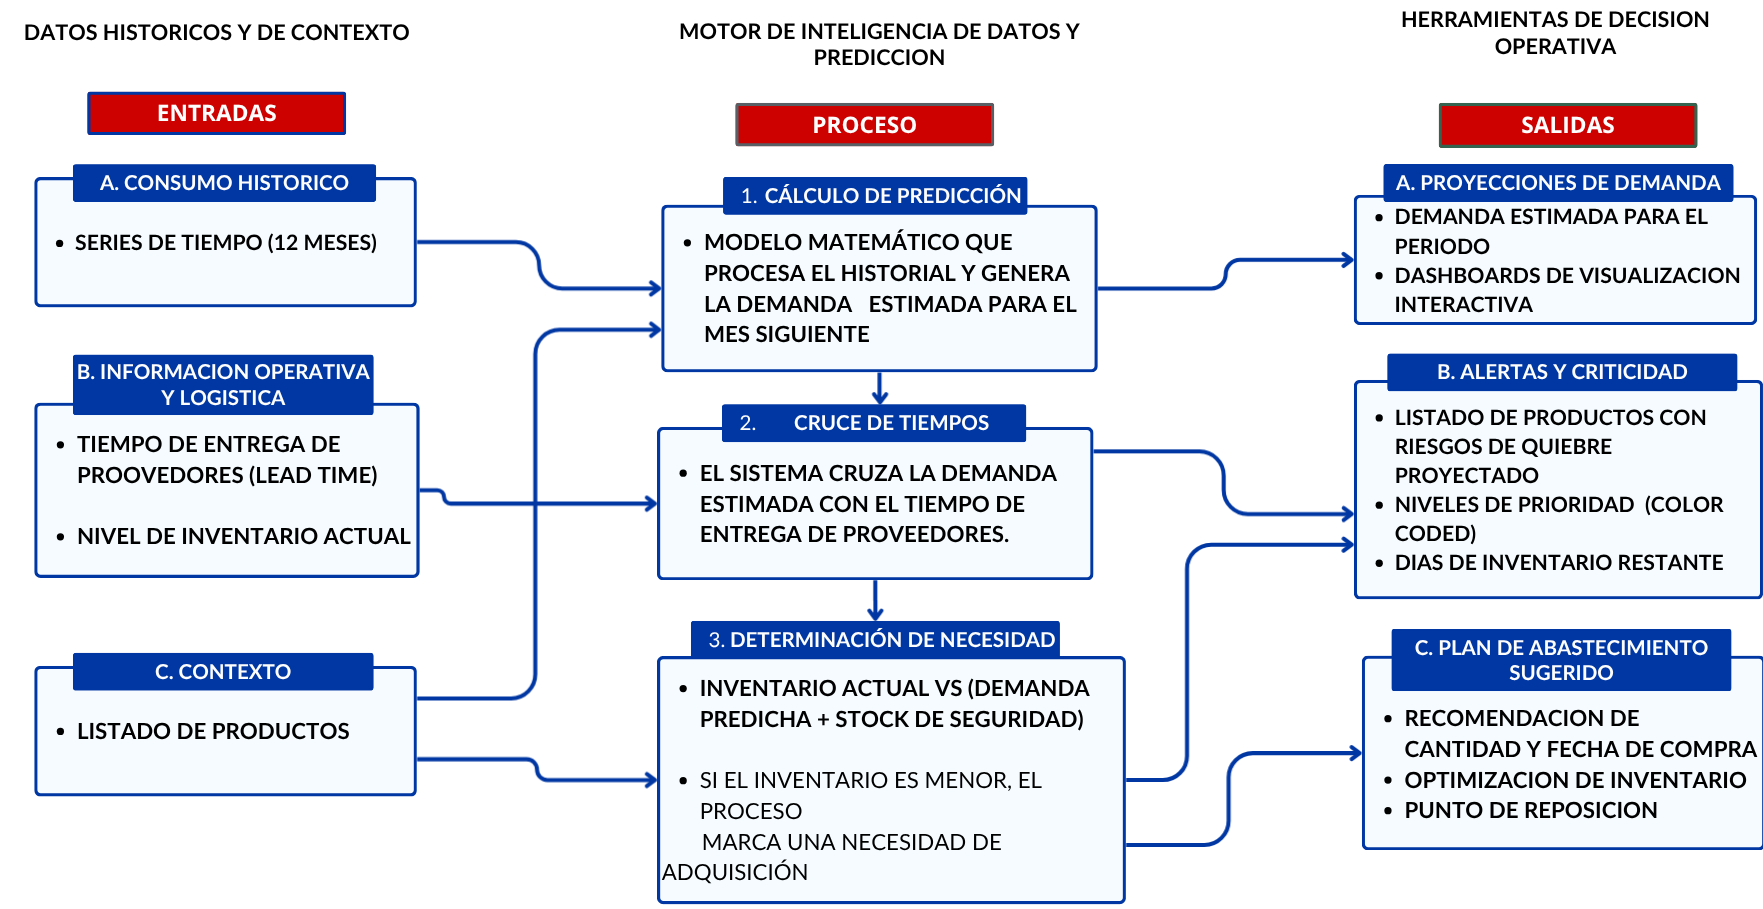
\includegraphics[width=1.0\textwidth]{templatefigures/entradas_salidas.png}
    \caption{Esquema detallado de entradas, proceso y salidas del sistema.}
\end{figure}